% !TeX root = mos-he.tex

%%%%%%%%%%%%%%%%%%%%%%%%%%%%%%%%%%%%%%%%%%%%%%%%%%%%%%%%%%%%%

\selectlanguage{hebrew}

\begin{center}
\textbf{\LARGE בעיות ופתרונות}
\end{center}

\addcontentsline{toc}{section}{\large בעיות ופתרונות}

\begin{prob}{מגרת הגרביים}{}{(The sock drawer)}

במגרה נמצאות גרביים אדומות וגרביים שחורות. אם נשלוף שתי גרביים בצורה אקראית
\textbf{ללא החזרה}
ההסתברות ששתיהן אדומות היא
$\frac{1}{2}$. 

\que{1}
מה המספר הקטן ביותר של גרביים שחורות שיכולות להיות במגרה? עבור מספר זה מה מספר הגרביים האדומות?

\que{2}
מה המספר 
\textbf{הזוגי}
הקטן ביותר של גרביים שחורות שיכולות להיות במגרה? עבור מספר זה מה מספר הגרביים האדומות?

\end{prob}
\solution{1}

\ans{1}
יהי
$r$
מספר הגרביים האדומות במגירה ויהי 
$b$
מספר הגרביים השחורות. 
$r\geq 2$
כי נתון שניתן לשלוף שתי גרביים אדומות, ו-%
$b\geq 1$
אחרת ההסתברות של שליפת שתי גרביים אדומות היתה 
$1$.
נכפיל את ההסתברויות של שתי השליפות:
\begin{equation}\label{eq.1-a}
P(\textrm{אדומים שניים})=\frac{r}{r+b} \cdot \frac{(r-1)}{(r-1)+b} = \frac{1}{2}\,.
\end{equation}
נפשט ונקבל משוואה ריבועית עבור המשתנה 
$r$:
\begin{equation}\label{eq.quad-for-r}
r^2-r(2b+1)-(b^2-b)=0\,.
\end{equation}
$r,b$
שנייהם מספרים שלמים חיוביים ולכן הדיסקרימיננט חייב להיות ריבוע של מספר שלם:
\begin{equation}\label{eq.discriminant}
(2b+1)^2+4(b^2-b)=8b^2+1
\end{equation}
הדיסקרימיננט הוא ריבוע כאשר 
$b=1$
(הערך הקטן ביותר). ממשוואה%
~\ref{eq.quad-for-r}
מתקבל 
$r=3$,
כאשר אנו דוחים את הפתרון 
$r=0$
כי
$r\geq 2$.
סכום מספר הגרביים הוא 
$4$.

בדיקה:
$\frac{3}{4}\cdot\frac{2}{3}=\frac{1}{2}$.

\medskip

\ans{2}
נבדוק מספרים שלמים חיובים זוגיים עבור 
$b$
כדי למצוא את הקטן ביותר עבורו הדיסקרימיננט הוא ריבוע:
\begin{displaymath}
\renewcommand{\arraystretch}{1}
\begin{array}{r|r|r}
b&8b^2+1&\sqrt{8b^2+1}\\
\hline
2&33&5.74\\
4&129&11.36\\
\mathbf{6}&\mathbf{289}&\mathbf{17}
\end{array}
\end{displaymath}
עבור
$b=6$ 
הערך של 
$r$
הוא
$15$
שמתקבל על ידי פתרון משוואה%
~\ref{eq.quad-for-r}.

בדיקה:
$\frac{15}{21}\cdot\frac{14}{20}=\frac{1}{2}$.

\newpage

\solution{2}

\ans{1}
האם אי-שוויון זה נכון?
\begin{equation}\label{eq.1-b}
\frac{r}{r+b} \stackrel{?}{>} \frac{r-1}{(r-1)+b}\,.
\end{equation}
$r\geq 2, b\geq 1$
ולכן שני המכנים חיוביים וניתן להכפיל את שני הצדדים:
\begin{eqn}
r(r-1+b)&\stackrel{?}{>}&(r-1)(r+b)\\
r^2-r+rb&\stackrel{?}{>}&r^2-r+rb-b\\
b&\stackrel{?}{>}&0\,.
\end{eqn}
$b>1$
כך שמשווה%
~\ref{eq.1-b}
נכונה.

לפי משוואות%
~\ref{eq.1-a}, \ref{eq.1-b}:
\begin{equation}\label{eq.1-c}
\left(\frac{r}{r+b}\right)^2 = \frac{r}{r+b} \cdot\frac{r}{r+b} > \frac{r}{r+b} \cdot \frac{r-1}{(r-1)+b} = \frac{1}{2}\,,
\end{equation}
ובאופן דומה:
\begin{equation}\label{eq.1-d}
\left(\frac{r-1}{(r-1)+b}\right)^2  = \frac{r-1}{(r-1)+b}\cdot \frac{r-1}{(r-1)+b}<  \frac{r}{r+b} \cdot \frac{r-1}{(r-1)+b} = \frac{1}{2}\,.
\end{equation}
המכנה
$r+b$
שונה מאפס ולכן ניתן לחשב שורש ריבועי ולפשט את משוואה%
~\ref{eq.1-c}:
\begin{eqn}
\frac{r}{r+b}  &>& \sqrt{\frac{1}{2}}\\
r&>&\frac{b}{\sqrt{2}-1}\\
r&>&\frac{b}{\sqrt{2}-1}\cdot\frac{\sqrt{2}+1}{\sqrt{2}+1}\\
r&>&b(\sqrt{2}+1)\,.
\end{eqn}
באופן דומה עבור משוואה%
~\ref{eq.1-d}:
\begin{eqn}
\frac{r-1}{(r-1)+b}&<&\sqrt{\frac{1}{2}}\\
r-1 &<& \frac{b}{\sqrt{2}-1}\\
r-1&<&b(\sqrt{2}+1)\,.
\end{eqn}
משתי המשוואות נקבל:
\begin{equation}\label{eq.inequalities}
r-1<(\sqrt{2}+1)b<r\,.
\end{equation}
עבור 
$b=1$
מתקבל
$2.141 < r< 3.141$
ו-%
$b=1,r=3$
הוא פתרון.

\ans{2} 
נבדוק מספרים זוגיים עבור
$b$:
\begin{displaymath}	
\renewcommand{\arraystretch}{1}
\begin{array}{r|ccc|c|c}
b& (\sqrt{2}+1)b&<r<& (\sqrt{2}+1)b+1&r&P(\textrm{שתי אדומות})\\
\hline
2&4.8&<r<&5.8&5&0.4762\\
4&9.7&<r<&10.7&10&0.4945\\
6&14.5&<r<&15.5&
15&0.5000
\end{array}
\end{displaymath}
\L{Mosteller}
מעיר שקיים קשר בין בעיה זו לתורת המספרים ומביא פתרון נוסף:
$b=35,r=85$.


\medskip
\sml{}
\selectlanguage{english}
\begin{verbatim}
Expectation of both red  = 0.5000
Average of both red for (red =  3, black =  1) = 0.5053
Average of both red for (red = 15, black =  6) = 0.5013
Average of both red for (red = 85, black = 35) = 0.4961
\end{verbatim}
\selectlanguage{hebrew}

\textbf{הערה}

בשני הפתרונות אנחנו לא מוכיחים תנאי
\emph{מספיק}
עבור הערכים של 
$r,b$.
בפתרון~
$1$
פיתחנו תנאי הכרחי: לפי משוואה%
~\ref{eq.discriminant}
הדיסקרימיננט חייב להיות מספר שלם, ומחפשים ערכים של 
$b$
שעומדים בדרישה זו. בפתרון~$2$ התנאי ההכרחי הוא ש-%
$r,b$
מספקים את האי-שוויונות במשוואה%
~\ref{eq.inequalities}
ואז חיפשנו ערכים שעומדים בדרישה זו. כתבתי תכנית קצרה לחפש פתרונות בטווח 
$[1,50]$.
התוצאות  עבור ערכים מסביב ל-%
$35$
הן:
\[
\renewcommand{\arraycolsep}{12pt}
\begin{array}{r|r|r|r}
\multicolumn{1}{c|}{r}&
\multicolumn{1}{c|}{b}&
\multicolumn{1}{c|}{\sqrt{8b^2+1}}&
\multicolumn{1}{c}{P(\textrm{אדומות שתי})} \\\hline
32 & 78  & 90.52 & 0.500917\\
33 & 80  & 93.34 & 0.499368\\
34 & 83  & 96.17 & 0.501474\\
35 & 85  & 99.00 & 0.500000\\
36 & 87  &101.83 & 0.498601\\
37 & 90  &104.66 & 0.500562
\end{array}
\]
הנה הפתרונות עבור
$b<10^6$:
\[
\begin{array}{r@{\hspace{2em}}r}
\textrm{שחורות} & \textrm{אדומות}\\\hline
1 & 3 \\
6 & 15\\
35 &  85\\
204 &  493\\
1189 &  2871\\
6930 & 16731\\
40391 &  97513\\
235416 & 568345
\end{array}
\]

%%%%%%%%%%%%%%%%%%%%%%%%%%%%%%%%%%%%%%%%%%%%%%%%%%%%%%%%%%%%%

\newpage

\begin{prob}{נצחונות עוקבים}{}{(Successive wins)}

אתה משחק סדרה של שלושה משחקים נגד שני יריבים ואתה זוכה בסדרה אם אתה מנצח שני משחקים לפחות מתוך השלושה. ההסתברות שאתה מנצח במשחק נגד שחקן 
$P_1$
היא
$p_1$
וההסתברות שאתה מנצח במשחק נגד שחקן 
$P_2$
היא
$p_2$.
נתון ש-%
$p_1>p2$.
באיזה המתסריטים שלהן יש סיכוי גדול יותר לזכות בסדרה?
\begin{itemize}
\item 
אתה משחק נגד 
$P_1,P_2,P_1$
בסדר זה.
\item
אתה משחק נגד
$P_2,P_1,P_2$
בסדר זה.
\end{itemize}
\end{prob}
\solution{1}

אתה זוכה אם: (א) אתה מנצח בשני השחקים הראשונים ומפסיד בשלישי, (ב) אתה מפסיד את המשחק הראשון ומנצח במשחק השני ובמשחק השלישי. (ג) אתה מנצח בשלושת המשחקים.

תהי
$p_{121}$
ו-%
$p_{212}$
ההסתברויות שאתה זוכה בשני סדרי המשחק:
\begin{eqn}
p_{121}&=&p_1p_2(1-p_1) + (1-p_1)p_2p_1 + p_1p_2p_1\\
p_{212}&=&p_2p_1(1-p_2) + (1-p_2)p_1p_2 + p_2p_1p_2\,.
\end{eqn}
קיים סיכוי גדול יותר לזכות בתסריט הראשון אם 
$p_{121}>p_{212}$,
כלומר, אם:
\begin{eqn}
p_1p_2(1-p_1) + (1-p_1)p_2p_1 + p_1p_2p_1 &\stackrel{?}{>}& 
p_2p_1(1-p_2) + (1-p_2)p_1p_2 + p_2p_1p_2\\
-p_1 & \stackrel{?}{>}& -p_2\\
p_2&\stackrel{?}{>}&p_1\,.
\end{eqn}
נתון ש-%
$p_1>p_2$
לכן כדאי לבחור את התסריט השני.

\solution{2}

הפתרון לא-איטואיטיבי. לפי האינטואיציה, כדאי לבחור לשחק שני משחקים נגד 
$P_1$
ואחד נגד
$P_2$
כי יש סיכוי גבוה יותר לנצח משחק נגד
$P_1$.
אולם, הדרך היחידה לנצח את הסדרה היא בנצחון ב-%
\textbf{משחק האמצעי},
ולכן, כדאי לשחק את המשחק האמצעי נגד 
$P_1$,
כי יש סיכוי גבוה יותר לנצח אותו.

\sml{}

\selectlanguage{english}
\begin{verbatim}
For p1 = 0.6, p2 = 0.5
Proportion of P121 wins = 0.4166
Proportion of P212 wins = 0.4473
For p1 = 0.6, p2 = 0.4
Proportion of P121 wins = 0.3300
Proportion of P212 wins = 0.3869
For p1 = 0.6, p2 = 0.2
Proportion of P121 wins = 0.1625
Proportion of P212 wins = 0.2141
\end{verbatim}

\selectlanguage{hebrew}
הסבר למה סכום היחסים אינו 
$1$.

%%%%%%%%%%%%%%%%%%%%%%%%%%%%%%%%%%%%%%%%%%%%%%%%%%%%%%%%%%%%%

\begin{prob}{המושבע קל הדעת}{}{(The flippant juror)}

קיימות שתי אפשרויות להגיע להכרעה: (א) פאנל של שלושה מושבעים המורכב משני מושבעים שמקבלים החלטה בלתי-תלויה עם הסתברות של 
$p$
להגיע להחלטה הנכונה, ומושבע שלישי שמגיע להחלטה נכונה בהסתברות של
$1/2$.
ההכרעה הנכונה מתקבלת לפי הצבעת רוב. (ב) ההכרעה מתקבלת על ידי מושבע יחיד שיש לו הסתברות של 
$p$
להגיע להחלטה נכונה. באיזו אפשרות הסתברות גבוהה יותר להגיע להכרעה נכונה?
\end{prob}

\solution{}

הפאנל מגיע להכרעה נכונה אם שלושת המושבעים מגיעים להחלטה נכונה או אם כל שני מושבעים מגיעים להחלטה נכונה. ההסתברות היא:
\[
P(\textrm{החלטה נכונה})=
\overbrace{\left(p\cdot p\cdot\frac{1}{2}\right)}^{\textrm{נכונים שלושה}}+\;\;\overbrace{\left(p(1-p)\cdot\frac{1}{2}+(1-p)p\cdot\frac{1}{2}+p\cdot p\cdot\frac{1}{2}\right)}^{\textrm{ שלושה מתוך נכונים שניים}}=p\,,
\]
כך שאין הבדל בין שתי האפשרויות.

\textbf{Simulation}
\selectlanguage{english}
\begin{verbatim}
Prediction: probabilities of (a) and (b) are equal
For p = 0.25, proportion correct of (a) = 0.5019, (b) = 0.5046
For p = 0.50, proportion correct of (a) = 0.5072, (b) = 0.4970
For p = 0.75, proportion correct of (a) = 0.5062, (b) = 0.5040
\end{verbatim}
\selectlanguage{hebrew}

%%%%%%%%%%%%%%%%%%%%%%%%%%%%%%%%%%%%%%%%%%%%%%%%%%%%%%%%%%%%%

\begin{prob}{ניסוים עד להצלחה הראשונה}{}{(Trials until first success)}

\label{p.four}
מה התוחלת של מספר ההטלות של קוביה עד שמופיע $6$?
\end{prob}

\solution{1}

ההסתברות שההטלה ה-%
$i$
תהיה ההופעה הראשונה של 
$6$
היא ההסתברות שב-%
$i-1$
הטלות יופיע אחד מחמשת המספרים האחרים כפול ההסתברות שבהטלה ה-%
$i$
יופיע 
$6$.

נפשט את הסימון:
$p=1/6$,
$P=P(i\;\textrm{בהטלה}\;6\;\textrm{של ראשונה הופעה})$,
$E=E(6\; \textrm{של ראשונה הטלה})$.
אזי:
\begin{eqn}
\nonumber{}P&=&(1-p)^{i-1}p\\
\label{eq.expectation}
E&=&1p(1-p)^0 + 2p(1-p)^1+ 3p(1-p)^2+ 4p(1-p)^3 +\cdots =\sum_{i=1}^{\infty} ip(1-p)^{i-1}\,.
\end{eqn}
ללא ה-
$i$
הסכום הוא ההסתברות של הטלה של $6$ בסופי של דבר:
\begin{equation}\label{eq.geo}
P(6\;\textrm{של דבר של בסופו הטלה})= \sum_{i=1}^{\infty} p(1-p)^{i-1}=p\cdot\frac{1}{1-(1-p)}=1\,,
\end{equation}
שהיא לא תוצאה מפתיעה.

ניתן לחשב את התוחלת כך:
\[
\begin{array}{llllllllll}
E&=&p(1-p)^0 &+& p(1-p)^1&+& p(1-p)^2&+& p(1-p)^3 &+\cdots \\
& & &&p(1-p)^1&+& p(1-p)^2&+& p(1-p)^3 &+\cdots \\
&  &&&& &p(1-p)^2&+& p(1-p)^3 &+\cdots \\
&&&&&&&&p(1-p)^3 &+\cdots
\end{array}
\]
השורה הראשונה היא סכום הסדרה ההנדסית ממשוואה%
~\ref{eq.geo}
שהוא
$1$.
השורה השנייה היא אותה סדרה הנדסית עם איבר ראשון 
$p(1-p)$
ולכן הסכום הוא:
\[
\frac{p(1-p)}{1-(1-p)}=1-p\,.
\]
באופן דומה, סכום השורה השלישית הוא
$(1-p)^2$ 
וסכום השורה ה-%
$i$
הוא
$(1-p)^{i-1}$.
לכן התוחלת היא סכום הסידרה ההנדסית:
\[
E= 1 + (1-p) + (1-p)^2 + (1-p)^3 + \cdots= \frac{1}{1-(1-p)}=\frac{1}{p}=6\,.
\]

\solution{2}

הכפל את משוואה%
~\ref{eq.expectation}
ב-%
$1-p$
והחסר את תוצאה מאותה משוואה. התוצאה היא הסדרה ההנדסית במשוואה%
~\ref{eq.geo}:
\[
\begin{array}{rclcl}
E&=&p(1-p)^0 &+&2p(1-p)^1+ 3p(1-p)^2+ 4p(1-p)^3 +\cdots\\
E\cdot(1-p)&=&&&p(1-p)^1 + 2p(1-p)^2+ 3p(1-p)^3 +\cdots \\
E\cdot(1-(1-p)) &=& p &+& p(1-p)^1 + p(1-p)^2 + p(1-p)^3 +\cdots\\
&=&1\\
E&=&1/p=6\,.
\end{array}
\]

\solution{3}

נתייחס להטלה הראשונה בנפרד משאר ההטלות. אם בהטלה הראשונה מופיע 
$6$
(בהסתברות
$p$)
הטלה אחת מספיקה. אחרת, אם בהטלה לא מופיע 
$6$
(הסתברות
$1-p$)
אזי ההטלות הבאות מרכיבות סדרה זהה לסדרה המקורית שהתוחלת שלה היא
$E$.
לכן התוחלת היא:
\begin{eqn}
E &=& 1\cdot p + (E+1)(1-p)\\
E&=&\disfrac{1}{p}=6\,.
\end{eqn}

\newpage

\sml{}

\selectlanguage{english}
\begin{verbatim}
Expectation of first success = 6
Average of first success     = 6.0161
\end{verbatim}
\selectlanguage{hebrew}

%%%%%%%%%%%%%%%%%%%%%%%%%%%%%%%%%%%%%%%%%%%%%%%%%%%%%%%%%%%%%

\begin{prob}{מטבע בריבוע}{}{(Coin in a square)}

\que{1}
מטילים מטבע על רשת (ללא גבולות) של ריבועים בגודל אחיד. המטבע נוחתת על הרשת בצורה אקראית כאשר למרכז המטבע מתפלגות אחידה בתוך ריבוע.

נתון ריבוע עם צלע באורך 
$8$
ומטבע עם רדיוס
$3$,
מה ההסתברות שהמטבע נוחתת כולה בתוך הריבוע?

\que{2}
בכל הטלה אתה מרוויח 
$5$
אם המטבע נוחתת בתוך ריבוע ומפסיד
$1$
אם היא נוגעת בצלע של ריבוע. מה תוחלת הרווח לכל הטלה?

\que{3} 
פתח נוסחה להסתברות שהמטבע נוחתת בתוך ריבוע אם אורך הצלע הוא 
$a$
ורדיוס המטבע הוא
$r$
כאשר
$r<a/4$.
\end{prob}

\solution{}

\ans{1}
\ref{f.coins1}
מראה ריבוע עם אורך צלע 
$8$
וארבעה מעגלים בקוטר 
$3$
חסומים על ידי פינות הריבוע. מרכזי המעגלים מרכיבים ריבוע פנימי שאורך הצלע שלו הוא
$2$.
כל מטבע שמרכזה מחוץ לריבוע תחתוך צלע של הריבוע החיצוני. למיקום של מרכז המטבע התפלגות אחידה ולכן ההסתברות שהמטבע נוחתת בתוך הריבוע היא היחס בין שטח הריבוע הפנימי לשטח הריבוע החיצוני:
\[
P(\textrm{הריבוע בתוך נוחתת המטבע})=\frac{2\cdot 2}{8\cdot 8} =\frac{1}{16}=0.0625\,.
\]
\begin{figure}[tb]
\begin{center}
\begin{subfigure}{.43\textwidth}
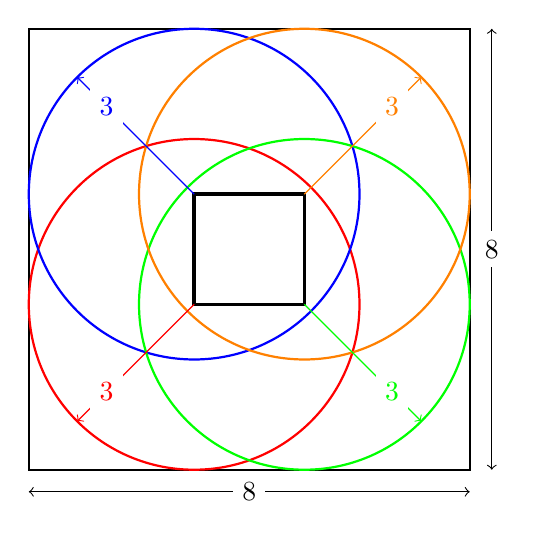
\begin{tikzpicture}[scale=.7]
\coordinate (c1) at (3,3);
\coordinate (c2) at (3,5);
\coordinate (c3) at (5,3);
\coordinate (c4) at (5,5);
\draw[very thick] (c1) -- (c3) -- (c4) -- (c2) -- cycle;
\draw[thick] (0,0) rectangle +(8,8);
\draw[color=red,thick] (c1) circle[radius=3];
\draw[color=blue,thick] (c2) circle[radius=3];
\draw[color=green,thick] (c3) circle[radius=3];
\draw[color=orange,thick] (c4) circle[radius=3];
\vertexcolor{c1}{red};
\vertexcolor{c2}{blue};
\vertexcolor{c3}{green};
\vertexcolor{c4}{orange};
\draw[<->] (0,-.4) -- node[fill=white] {$8$} (8,-.4);
\draw[<->] (8.4,0) -- node[fill=white] {$8$} (8.4,8);
\draw[->,red] (3,3) -- node[near end,fill=white] {$3$} +(-135:3);
\draw[->,blue] (3,5) -- node[near end,fill=white] {$3$} +(135:3);
\draw[->,green] (5,3) -- node[near end,fill=white] {$3$} +(-45:3);
\draw[->,orange] (5,5) -- node[near end,fill=white] {$3$} +(45:3);
\end{tikzpicture}
\caption{מטבעות בתוך הריבוע}\label{f.coins1}
\end{subfigure}
\hspace{3em}
\begin{subfigure}[b]{.43\textwidth}
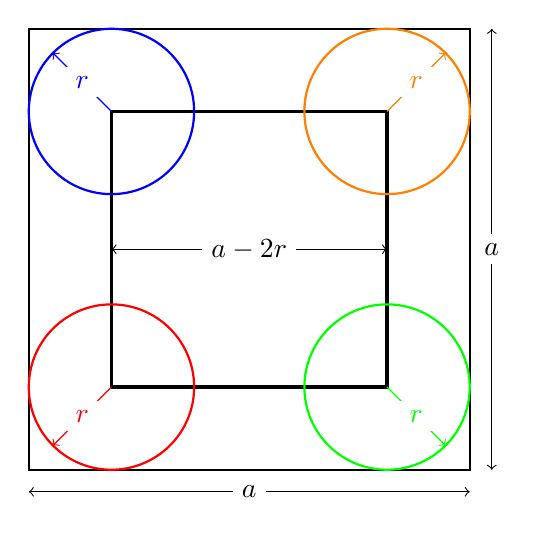
\begin{tikzpicture}[scale=.7]
\coordinate (c1) at (1.5,1.5);
\coordinate (c2) at (1.5,6.5);
\coordinate (c3) at (6.5,1.5);
\coordinate (c4) at (6.5,6.5);
\draw[very thick] (c1) -- (c3) -- (c4) -- (c2) -- cycle;
\draw[thick] (0,0) rectangle +(8,8);
\draw[color=red,thick] (c1) circle[radius=1.5];
\draw[color=blue,thick] (c2) circle[radius=1.5];
\draw[color=green,thick] (c3) circle[radius=1.5];
\draw[color=orange,thick] (c4) circle[radius=1.5];
\vertexcolor{c1}{red};
\vertexcolor{c2}{blue};
\vertexcolor{c3}{green};
\vertexcolor{c4}{orange};
\draw[<->] (0,-.4) -- node[fill=white] {$a$} (8,-.4);
\draw[<->] (8.4,0) -- node[fill=white] {$a$} (8.4,8);
\draw[->,red] (1.5,1.5) -- node[fill=white] {$r$} +(-135:1.5);
\draw[->,blue] (1.5,6.5) -- node[fill=white] {$r$} +(135:1.5);
\draw[->,green] (6.5,1.5) -- node[fill=white] {$r$} +(-45:1.5);
\draw[->,orange] (6.5,6.5) -- node[fill=white] {$r$} +(45:1.5);
\draw[<->] (1.5,4) -- node[fill=white] {$a-2r$} (6.5,4);
\end{tikzpicture}
\caption{מטבעות בתוך ריבוע גדול}\label{f.coins2}
\end{subfigure}
\end{center}
\end{figure}

\ans{2}
\[
E(\textrm{רווח לכל הטלה})=5\cdot\frac{1}{16}\,+\,(-1)\cdot\frac{15}{16}=-\frac{10}{16}=-0.625\,.
\]

\ans{3}
\ref{f.coins2}
מראה ארבעה מעגלים חסומים על ידי פינות הריבוע. הצלע של הריבוע הפנימית הוא 
$a-2r$
ולכן:
\[
P(\textrm{המעגל בתוך נוחתת המטבע})=\frac{(a-2r)^2}{a^2}\,.
\]

\sml{}
\selectlanguage{english}
\begin{verbatim}
For side = 8, radius = 1:
Probability of landing within the square = 0.5625
Proportion landing within the square     = 0.5704
For side = 8, radius = 2:
Probability of landing within the square = 0.2500
Proportion landing within the square     = 0.2481
For side = 8, radius = 3:
Probability of landing within the square = 0.0625
Proportion landing within the square     = 0.0639
For side = 8, radius = 4:
Probability of landing within the square = 0.0000
Proportion landing within the square     = 0.0000
\end{verbatim}
\selectlanguage{hebrew}

%%%%%%%%%%%%%%%%%%%%%%%%%%%%%%%%%%%%%%%%%%%%%%%%%%%%%%%%%%%%%

\begin{prob}{הטלת מזל}{}{(Chuck-a-luck)}

בחר מספר 
$n$
בין 
$1$
ל-%
$6$
והטל שלוש קוביות. אם לא מופיע
$n$
על אף קוביה אתה מפסיד
$1$;
אם 
$n$
מופיע על קוביה אחת אתה מרוויח
$1$;
אם 
$n$
מופיע על שתי קוביות אתה מרוויח
$2$;
אם 
$n$
מופיע על כל שלושת הקוביות אתה מרוויח 
$3$.
מה התוחלת של הרווח?
\end{prob}

\solution{}

תהי 
$P(k)$
ההסתברות ש-%
$n$
מופיע על 
$k$
קוביות. אזי:
\[
E(\textrm{הטלה לכל רווח})=-1 P(0) + 1 P(1) + 2 P(2) + 3 P(3)\,.
\]
ההטלות של שלושת הקוביה הן בלתי-תלויות ולכן:
\begin{eqn}
E(\textrm{הטלה לכל רווח}) &=& 
-1\dischoose{3}{0}\left(\frac{1}{6}\right)^0\left(\frac{5}{6}\right)^3
+1\dischoose{3}{1}\left(\frac{1}{6}\right)^1\left(\frac{5}{6}\right)^2+\\
&&\;\;\;2{3\choose 2}\left(\frac{1}{6}\right)^2\left(\frac{5}{6}\right)^1+
3\dischoose{3}{3}\left(\frac{1}{6}\right)^3\left(\frac{5}{6}\right)^0\\
&=& \frac{1}{216}(-125+75+30+3)\\
&=&-\frac{17}{216}\approx -0.0787\,.
\end{eqn}

\sml{}
\selectlanguage{english}
\begin{verbatim}
Expectation of winnings = -0.0787
Average winnings        = -0.0724
\end{verbatim}
\selectlanguage{hebrew}

%%%%%%%%%%%%%%%%%%%%%%%%%%%%%%%%%%%%%%%%%%%%%%%%%%%%%%%%%%%%%

\begin{prob}{לרפא את המהמר הכפייתי}{}{(Curing the compulsive gambler)}

\label{p.roulette}
רולט
(\L{roulette})
הוא משחק מזל שמשחקים עם גלגל בעל 
$38$
כיסים ממוספרים:
$18$
אדומים,
$18$
שחורים ו-%
$2$
ירוקים.%
\footnote{ברולט אמריקאי נמצאים שני כיסים ירוקים וברולט אירופאי נמצא כיס ירוק אחד.}
מסובבים את הגלגל, זורקים כדור לתוך הגלגל ומחכים שהכדור ינחת באחד הכיסים. הכדור נוחת בכיס אקראי עם התפלגות אחידה. אתה מהמר 
$1$
שהכדור ינחת בכיס מסוים.%
\footnote{זה סוג ההימור היחיד שמשתמשים בו בבעיות בספר זה.}
הקזינו זוכה אם הכדור נוחת בכיס ירוק, אחרת אתה מרוויח 
$36$
אם המרת 
$1$
על מספר הכיס בו נוחת הכדור. למעשה הרווח נטו הוא
$35$
כי התגמול של
$36$
כולל החזרה של דמי ההימור.

\que{1}
מה תוחלת הרווח עבור 
$36$
סבבים של משחק ברולט?

\que{2}
חברך מציע להמר 
$20$
שאחרי 
$36$
סבבים אתה 
\textbf{תפסיד}
כסף. מה תוחלת הרווח בהתחשב ברווח או הפסד גם של המשחק וגם של ההימור עם חברך?
\end{prob}

\solution{}

\ans{1}
ההסתברות של ניצחון בסבב אחד היא
$1/38$
ולכן:
\begin{eqn}
E(\textrm{אחד בסבב רווח})&=&35\cdot \frac{1}{38} + (-1)\cdot\frac{37}{38} = -\frac{2}{38} \approx -0.0526\\
E(\textrm{סבבים}\;36\textrm{ב- רווח })&=&36\cdot -0.05266=-1.8947\,.
\end{eqn}

\ans{2}
נבדוק את ארבעת התוצאות של 
$36$
סבבים של רולט:
\begin{itemize}
\item
אם אתה מפסיד בכל הסבבים ההפסד הוא 
$36$.
\item
אם אתה זוכה בסבב אחד ומפסיד ב-%
$36$
סבבים אין רווח ואין הפסד.
\item
אם אתה זוכה בשני סבבים את מרוויח
$70$
ומפסיד
$34$
בשאר הסבבים כך שהרווח נטו הוא
$36$.
\item 
אם אתה זוכה ב-%
$k$
עבור
$2<k\leq 36$,
הרווח נטו הוא
$35k - (36-k)>0$.
\end{itemize}
לכן אתה מפסיד כסף רק אם אתה מפסיד את כל הסבבים:
\begin{eqnarray*}
P(\textrm{סבבים} \;36 \textrm{ב- מפסיד})&=&\left(\frac{37}{38}\right)^{36}\approx 0.3829\\
E(\textrm{סה"כ רווחים})&=&
\overbrace{-1.8947}^{\textrm{\small הסבבים כל של E}}+\;\;
\overbrace{-20\cdot 0.3829}^{\textrm{\small בהימור מפסיד}} \;+\; \overbrace{20\cdot 0.6171}^{\textrm{\small בהימור זוכה}} \approx 2.7904\,.
\end{eqnarray*}
ברור שכדאי להסכים להימור המוצע!

\sml{}
\selectlanguage{english}
\begin{verbatim}
Expectation of winning a round = -0.0526
Average winnings for a round   = -0.0593
\end{verbatim}
\selectlanguage{hebrew}
בסימולציה היתה שונות גדולה שהוקטנה כל ידי הרצת מיליון ניסויים.

%%%%%%%%%%%%%%%%%%%%%%%%%%%%%%%%%%%%%%%%%%%%%%%%%%%%%%%%%%%%%

\begin{prob}{קלפים מושלמים בברידג'}{}{(Perfect bridge hand)}

בחר באקראי 
$13$
קלפים מחפיסה של 
$52$
קלפים. מה ההסתברות שכולם מאותה סדרה?
\end{prob}

\solution{1}

יש
$\dischoose{52}{13}$
דרכים לבחור 
$13$
קלפים מסדרה אחת. מתוכן יש ארבע דרכים שכולם מסדרה אחת, ולכן:
\[
P(\textrm{סדרה מאותה קלפים}\;13\;\textrm{בחירת })=4\cdot \frac{13! \cdot 39!}{52!}\approx 6.2991\times 10^{-12}\,.
\]

\solution{2}

יש 
$52$
דרכים לבחור את הקלף הראשון. אח"כ יש 
$12$
דרכים לבחור את הקלף השני מאותה סדרה מתוך 
$51$
הקלפים שנשארו,
$11$
דרכים לבחור את הקלף השלישי, וכו'. מכאן:
\[
P(\textrm{סדרה מאותה קלפים}\;13\;\textrm{בחירת})=\frac{52}{52}\cdot \frac{12}{51}\cdot \frac{11}{50} \cdots  \frac{1}{40}= \frac{12!}{51!/39!}\approx 6.2991\times 10^{-12}\,.
\]

\sml{}

אין טעם להריץ סימולציה עם 
$52$
קלפים כי ההסתברות תהיה אפס כמעט בוודאות. הרצתי סימולציה עם חפיסה של 
$16$
קלפיםם ו-%
$4$
סדרות.
\selectlanguage{english}
\begin{verbatim}
Probability of perfect hand = 0.0022
Proportion perfect hand     = 0.0020
\end{verbatim}
\selectlanguage{hebrew}

%%%%%%%%%%%%%%%%%%%%%%%%%%%%%%%%%%%%%%%%%%%%%%%%%%%%%%%%%%%%%

\begin{prob}{משחק "קראפס"}{D}{(Craps)}

משחק ה-%
\L{craps}
הוא משחק עם זוג קוביות. בהטלה הראשונה אתה זוכה אם סכום המספרים הוא
$7$
או
$11$,
ואתה מפסיד אם הסכום הוא
$2$, $3$
או
$12$.
אם הסכום בהטלה הראשונה הוא
$n=4,5,6,8,9,10$ 
(נקרא "נקודה" 
\L{point}),
המשך להטיל את הקוביות עד שמופיעה הנקודה 
$n$
(ניצחון) או 
$7$
(הפסד).

\que{1} 
מה ההסתברות של המאורעות בהטלה הראשונה: ניצחון, הפסד, לא ניצחון ולא הפסד?

\que{2} 
מה ההסתברות לניצחון?
\end{prob}

\solution{1}

%%%%%%%%%%%%%%%%%%%%%%%%%%%%%%%%%%%%

\ans{1}
להסתברות של תוצאה בהטלה קוביה התפלגות אחידה וההטלות של שתי קוביות בלתי-תלויות, ולכן ההסתברות של כל תוצאה היא 
$1/36$.
מספר הדרכים לקבל כל אחד מהמאורעות (הסכום של זוג הקוביות) הוא:
\[
\begin{array}{rrrrrrrrrrr|l}
2 & 3 & 4 & 5 & 6 & 7 & 8 & 9 & 10 & 11 & 12&\textrm{סכום}\\\hline
 1 & 2 & 3 & 4 & 5 & 6 & 5 & 4 & 3 & 2 & 1&\textrm{זוגות}
\end{array}
\]
בהטלה הראשונה יש 
$8$
דרכים לקבל
$7$
או
$11$
וההסתברות לניצחון היא
$8/36$.
יש
$4$
דרכים לקבל
$2,3,12$
וההסתברות להפסד היא 
$4/36$.
ההסתברות לא לנצח ולא להפסיד בהטלה הראשונה היא:
\[
1 - \frac{8}{36} - \frac{4}{36} = \frac{24}{36}\,.
\]

%%%%%%%%%%%%%%%%%%%%%%%%%%%%%%%%%%%%

\ans{2}
נעיין בשני מקרים:
\begin{itemize}
\item 
הנקודה היא
$4$.
ההסתברות לנצח בהטלה השנייה ($4$) היא
$3/36$
וההסתברות להפסיד ($7$) היא
$6/36$.
ההסתברות לא לנצח ולא להפסיד היא
$1-(3/36)-(6/36)=27/36$.

\item
הנקודה היא $8$. ההסתברות לנצח בהטלה השנייה ($8$) היא
$5/36$
וההסתברות להפסיד ($7$) היא
$6/36$.
ההסתברות לא לנצח ולא להפסיד היא
$1-(5/36)-(6/36)=25/36$.
\end{itemize}
אנו רואים שחייבים לחשב את ההסתברות לנצח בנפרד עבור כל אחת מהנקודות 
$4,5,6,8,9,10$.
נפתח נוסחה כללית להסתברות.

תהי 
$P_n$
ההסתברות לנצח בהטלת הנקודה 
$n$
בהטלה ו-%
$Q_n$
ההסתברות לא לנצח ולא להפסיד בהטלה כלשהי. ניתן לחשב את
$W_n$,
ההסתברות לניצחון על ידי הטלת הנקודה 
$n$
\textbf{לאחר ההטלה הראשונה},
על ידי חיבור:
\begin{itemize}
\item 
ההסתברות להופעת הנקודה בהטלה השנייה. 
\item 
ההסתברות לא לנצח ולא להפסיד בהטלה השנייה וההסתברות להופעת הנקודה בהטלה השלישית.
\item 
ההסתברות לא לנצח ולא להפסיד בהטלה השנייה והשלישית וההסתברות להופעת הנקודה בהטלה הרביעית,
\item
$\cdots$
\end{itemize}
\vspace{-6ex}
\begin{eqn}
W_n&=&P_n + Q_n P_n + Q_n^2 P_n+ Q_n^3 P_n  + \cdots\\
&=&P_n\left(1+Q_n^1 + Q_n^2+ Q_n^3  + \cdots\right)\\
&=&P_n\left(\frac{1}{1-Q_n}\right)\,.
\end{eqn}
אתה מפסיד אם בהטלה כלשהי לאחר הראשונה מופיע 
$7$
עם הסתברות
$6/36$
ולכן:
\begin{eqn}
Q_n &=& (1-P_n)-(6/36)\\
W_n&=&\frac{P_n}{P_n+(6/36)}\,.
\end{eqn}
$W_n$
עבור ששת הנקודות היא:
\[
\renewcommand{\arraystretch}{2}
\begin{array}{lcccccc}
n   & 4 & 5 & 6 & 8 & 9 & 10 \\\hline
P_n & \disfrac{3}{36} & \disfrac{4}{36} & \disfrac{5}{36} & \disfrac{5}{36} & \disfrac{4}{36} & \disfrac{3}{36} \\
%1-Q_n & \disfrac{9}{36} & \disfrac{10}{36} & \disfrac{11}{36} & \disfrac{11}{36} & \disfrac{10}{36} & \disfrac{9}{36} \\
W_n & \disfrac{3}{9} & \disfrac{4}{10} & \disfrac{5}{11} & \disfrac{5}{11} & \disfrac{4}{10} & \disfrac{3}{9}
\end{array}
\]
נחשב את
$W$, 
ההסתברות לנצח, על ידי חיבור ההסתברות לנצח בהטלה הראשונה לסכום ההסתברויות לנצח על ידי הטלת נקודה כפול ההסתברות להופעת 
\textbf{אותה נקודה}
בהטלה הראשונה:
\begin{equation}\label{eq.9-a}
W=\frac{8}{36}+\sum_{n\in\{4,5,6,8,9,10\}} P_nW_n \approx 0.4929\,.
\end{equation}
שסיכוי שהקזינו יזכה במשחק אחד של 
\L{craps}
הוא רק
$0.5-0.4949\approx 0.5\%$
אבל חוק המספרי הגדולים מבטיח שבסופו של דבר הם ינצחו ואתה תפסיד!

%%%%%%%%%%%%%%%%%%%%%%%%%%%%%%%%%%%%

\solution{2}

\ans{2}
נעיין בסדרות ההטלות שלהן כאשר בכולן הנקודה היא
$4$:
\[
\begin{array}{rrrrrrrrrrr}
4 & 8 & 9 & 9 & 9 & 8 & 8 & 8 & 9 & 8 & 4\\
4 & 8 & 9 & 9 & 9 & 8 & 8 & 8 & 9 & 8 & 7\\
4 & 9 & 9 & 9 & 8 & 8 & 4
\end{array}
\]
המשחק מסתיים רק אם מטילים 
$4$
(ניצחון) או מטילים
$7$
(הפסד), כך שהופעות של 
$8$
או
$9$
לא משפיעות על התוצאה. מכאן שהסתברות לנצח היא ההסתברות המותנית שתופיע
$4$
אם נתון שכבר הופיע
$4$
או
$7$. 
יהי 
$f$
המאורע ש-%
$4$
מופיע ו-%
$s$
המאורע ש-%
$7$
מופיע. אזי:
\[
P(f|f\cup s) = \disfrac{P(f)\cap P(f\cup s)}{P(f\cup s)}=\disfrac{P(f)}{P(f\cup s)}=\disfrac{3/36}{(3+6)/36}=\disfrac{3}{9}\,,
\]
בדיוק הערך
$W_4$
בטבלה לעיל. כעת ניתן להשתמש במשוואה%
~\ref{eq.9-a}
כדי לחשב את
$W$.

השתמשנו בהסתברות בצורה סמויה בפתרון הראשון, כי 
$W_n$
היא הסתברות שמותנית בהופעת הנקודה
$n$
בהטלה הראשונה.

\sml{}
\selectlanguage{english}
\begin{verbatim}
Probability of winning = 0.4929
Proportion of wins     = 0.4948
\end{verbatim}
\selectlanguage{hebrew}

%%%%%%%%%%%%%%%%%%%%%%%%%%%%%%%%%%%%%%%%%%%%%%%%%%%%%%%%%%%%%

\refstepcounter{problem}  % 10. An experiment in personal taste

%%%%%%%%%%%%%%%%%%%%%%%%%%%%%%%%%%%%%%%%%%%%%%%%%%%%%%%%%%%%%

\refstepcounter{problem}  % 11. Silent cooperation

%%%%%%%%%%%%%%%%%%%%%%%%%%%%%%%%%%%%%%%%%%%%%%%%%%%%%%%%%%%%%

\refstepcounter{problem}  % 12. Quo vadis?

%%%%%%%%%%%%%%%%%%%%%%%%%%%%%%%%%%%%%%%%%%%%%%%%%%%%%%%%%%%%%

\begin{prob}{דילמת האסיר}{}{(The prisoner's dilemma)}

שלושה אסירים 
$A,B,C$
מועמדים לשחרור מוקדם. וועדת השחרורים תשחרר שניים מהם כך שהאפשריות הן
$\{A,B\}, \{A,C\}, \{B,C\}$
בהסתברות שווה של
$1/3$.
לכן ההסתברות ש-%
$A$
ישוחרר היא
$2/3$.
מפקד הכלא מוסר ל-% 
$A$
מידע נכון: את זהותו האסיר האחר שישוחרר 
$B$
או
$C$.
אם ל-%
$A$
נמסר ש-%
$B$
ישוחרר, מה ההסתברות שהוא ישוחרר גם כן?
\end{prob}

שלושת הפתרונות שלהלן דומות מאוד אבל השיטות לחישוב ההסתברויות המותנות שונות.

\solution{1}

ארבעת המאורעות האפשריים הם (איור%
~\ref{f.pp}):
\begin{description}
\item[$e_1$:] 
ל-%
$A$
נמסר ש-%
$B$
ישוחרר ו-%
$\{A,B\}$
ישוחררו.
\item[$e_2$:]
ל-%
$A$
נמסר ש-%
$C$
ישוחרר ו-%
$\{A,C\}$
ישוחררו.
\item[$e_3$:]
ל-%
$A$
נמסר ש-%
$B$
ישוחרר ו-%
$\{B,C\}$
ישוחררו.
\item[$e_4$:]
ל-%
$A$
נמסר ש-%
$C$
ישוחרר ו-%
$\{B,C\}$
ישוחררו.
\end{description}
ההסתברות של כל זוג להשתחרר שווה ולכן:
\[
P(e_1)=P(e_2)=P(e_3\cup e_4)=\frac{1}{3}\,.
\]
אם 
$\{B,C\}$
ישוחררו, יימסר ל-%
$A$
מידע נכון ש-%
$B$
או 
$C$
ישוחרר ובהסתברות שווה, ולכן
$P(e_3)=P(e_4)=1/6$.
ההסתברות המותנית ש-%
$A$
ישוחרר (מאורע
$e_1$)
בהינתן שנמסר ל-%
$A$
ש-%
$B$
ישוחרר (מאורע
$e_1\cup e_3$)
היא:
\[
P(e_1|e_1\cup e_3) = \frac{P(e_1\cap(e_1\cup e_3))}{P(e_1\cup e_3)}=\frac{P(e_1)}{P(e_1\cup e_3)}=\frac{1/3}{1/3+1/6}=\frac{2}{3}\,.
\]

\begin{figure}[tb]
\begin{center}
\begin{tikzpicture}
\coordinate (root) at (0,0);
\draw[thick,->] (root) -- node[above] {$1/3$} (4,2)
  coordinate(top) node[right] {$\{B,C\}$};
\draw[thick,->] (root)-- node[above] {$1/3$} (4,0)
   coordinate(middle) node[right] {$\{A,B\}$};
\draw[thick,->] (root)-- node[below,yshift=-3pt] {$1/3$} (4,-2)
  coordinate(bottom) node[right]  {$\{A,C\}$};
\draw[thick,->] ($(top)+(1.6,0)$) --
  node[above] {$1/2$} +(4,.6)
  coordinate(one) node[right] {$B$};
\draw[thick,->] ($(top)+(1.6,0)$) --
  node[below] {$1/2$} +(4,-.6)
  coordinate(two) node[right] {$C$};
\draw[thick,->] ($(middle)+(1.6,0)$) --
  node[below] {$1$}  +(4,0) 
  coordinate(three) node[right] {$B$};
\draw[thick,->] ($(bottom)+(1.6,0)$) --
  node[below] {$1$} +(4,0)
  coordinate(four) node[right] {$C$};
\node at ($(top)+(.5,1.8)$) {\R{אסירים שישוחררו}};
\node at ($(one)+(.45,1.2)$) {\R{מפקד מספר שישוחרר}};
\end{tikzpicture}
\selectlanguage{hebrew}
\caption{עץ לבעיית האסיר}\label{f.pp}
\end{center}
\end{figure}

%%%%%%%%%%%%%%%%%%%%%%%

\newpage

\solution{2}


ההסתברות המותנית ש-%
$A$
ישוחרר בהינתן ש-% 
$B$
ישוחרר היא:
\[
P(A|B) = \frac{P(A\cap B)}{P(B)} = \frac{1/3}{2/3}=\frac{1}{2}\,.
\]
אבל זאת 
\textbf{לא}
ההסתברות המותנית הנכונה. המידע החדש הוא
\textbf{שנמסר}
ל-%
$A$
ש-%
$B$
ישוחרר. יהי
$R_{AB}$
המאורע של-%
$A$
נמסר ש-%
$B$
ישוחרר, אזי:
\[
P(A|R_{AB}) = \frac{P(A\cap R_{AB})}{P(R_{AB})}
\]
המידע על שחרורו של
$B$
הוא אמת ולכן:
\[
P(A\cap R_{AB})=P(\{A,B\})=\disfrac{1}{3}\,.
\]
אם 
$\{B,C\}$
ישוחררו שההסתברות היא
$1/2$
שמפקד יספר ל-%
$A$
ש-%
$B$
ישוחרר וגם ההסתברות היא
$1/2$
שהמפקד יספר ש-%
$C$
ישוחרר, ולכן:
\begin{eqnarray*}
P(R_{AB})&=&P(\{A,B\})+\disfrac{1}{2}\cdot P(\{B,C\})=\disfrac{1}{3}+\disfrac{1}{2}\cdot \disfrac{1}{3}=\disfrac{1}{2}\\
P(A|R_{AB}) &=& \frac{P(A\cap R_{AB})}{P(R_{AB})} = \disfrac{1/3}{1/2}=\disfrac{2}{3}\,.
\end{eqnarray*}

%%%%%%%%%%%%%%%%

\solution{3}

$P(A)=2/3$
נתונה. 
$P(R_{AB}|A)=1/2$
כי אם 
$A$
ישחורר,
$B$
או
$C$
ישוחרר בהסתברות שווה. חישבנו ש-%
$P(R_{AB})=1/2$.
לפי חוק בייס:
\[
P(A|R_{AB})= \frac{P(R_{AB}|A)\,P(A)}{P(R_{AB})} = \displaystyle\frac{(1/2)(2/3)}{1/2}=\displaystyle\frac{2}{3}\,.
\]

%%%%%%%%%%%%%%%%

%\medskip\textbf{\Large הבעיה של מונטי הול \normalsize \L{(Monty Hall Problem)}}
%
%נציג כאן את הבעיה של מונטי הול (שלא מופיע בספר) כדי להראות את הקשר  בינה לבין בעיית האסיר.
%
%דיונים רבים בספרות נובעים מפרשנויות לניסוח הבעיה ולכן כדי למנוע בלבול אפרט לפרטי פרטים את כללי המשחק ואת ההנחות שלעתים נשארו סמויות:
%
%\begin{enumerate}
%\item
%בשעשועון בטלוויזיה המתחרה ניצב לפני שלוש דלתות סגורות. מאחרי כל אחת מהדלתות נמצא אחד הפרסים שהם מכונית אחת ושתי עזים.
%\item
%המתחרה מעדיף לזכות במכונית ולא בעז!%
%\footnote{%
%לא מצאתי הנחה סמויה זו כתובה בספרות אבל אם רוצים לדייק כדאי להציף אותה.}
%\item
%מיקום כל פרס הוא אקראי בהתפלגות אחידה.
%\item
%המנחה יודע את המיקום של כל אחד מהפרסים. 
%\item
%המתחרה חייב לבחור דלת אחת.
%\item
%לפני שמגלים למתחרה איזה פרס נמצא מאחורי הדלת שבחר, המנחה חייב לפתוח את אחת הדלתות שמאחוריהן נמצאות העזים. קיימות שתי אפשרויות:
%\begin{itemize}
%\item
%אם המתחרה בחר בדלת עם המכונית, הבחירה של המנחה בין שתי הדלתות האחרות היא אקראית בהתפלגות אחידה.
%\item
%אם המתחרה בחר בדלת עם עז, המנחה חייב לפתוח את הדלת עם העז השניה.
%\end{itemize}
%\item
%לאחר פתיחת הדלת המתחרה חייב להחליט אם להישאר עם הבחירתו המקורית או לשנות אותה ולבחור בדלת השניה שלא נפתחה.
%\item
%המנחה פותח את הדלת שנבחרה והמתחרה זוכה בפרס שנמצא שם.
%\end{enumerate}
%מה האסטרטגיה העדיפה עבור המתחרה: להישאר עם הבחירה המקורית או לשנות אותה?
%
%לפי פתרון שכיח ההסתברות שהמכונית נמצאת מאחורי הדלת המקורית משתנה מ-%
%$1/3$
%ל-%
%$1/2$
%כי המכונית נמצאת מאחורי אחת משתי הדלתות שעדיין סגורות, ולכן לא משנה אם המתחרה בוחר להישאר עם החלטתו או לשנותה. פתרון זה 
%\textbf{שגוי}
%כי אין כאן שני ניסויים בלתי-תלויים. לאחר פתיחת הדלת, המנחה לא
%מטיל מטבע כדי להחליט מחדש איפה לשים את המכונית ואיפה לשים את העז.
%
%נניח ששינו את כללי המשחק כך שהמתחרה 
%\textbf{לא}
%רשאי לשנות את החלטתו! ההסתברויות לא משתנות: ההסתברות לזכות במכונית נשארת
%$1/3$
%והסתברות לזכות בעז נשארת
%$2/3$.
%מצב זה שקול לבעיית האסיר כי האסיר 
%$A$
%לא רשאי לשנות את ההחלטה מי ישוחרר, ולכן לא משנה מה אומרים לו. עם הכללים החדשים לא משנה איזו דלת המנחה פותח, המתחרה לא יכול לעשות כלום.
%
%בעיית מונטי הול שונה. הכלל שהמתחרה רשאי לשנות את החלטתו היא הסיבה היחידה שיש משמעות לפתיחת הדלת. שוב, ההסתברויות לא משתנות: הההסתברות שהמכונית נמצאת האחורי הדלת שנבחרה בהחלטה המקורית היא
%$1/3$,
%והסתברות שהיא נמצאת האחורי שתי הדלתות האחרות היא
%$2/3$.
%אבל כעת הסתברות
%$2/3$
%"מרוכזת" בדלת אחת, זו שהמנחה לא פתח, ולכן, המתחרה יכול להכפיל את סיכוייו לזכות במכונית מ-%
%$1/3$
%ל-%
%$2/3$
%על ידי שינוי ההחלטה.
%
%%%%%%%%%%%%%%%%%%
%
%\sml{}
%
%אין סימולציה לבעיית האסירים כי הבעיה שואלת אם ההסתברות משתנה לאור ידע חדש, אבל הראנו שאין שינוי. הנה תוצאות הסימולציה של בעיית מונטי הול עבור 
%$10000$
%משחקים:
%
%\selectlanguage{english}
%\begin{verbatim}
%Wins when staying with original door = 0.3311
%Wins when changing door              = 0.6689
%\end{verbatim}
%\selectlanguage{hebrew}


%%%%%%%%% Old version commented out %%%%%

\begin{comment}

\begin{prob}{דילמת האסיר}{}{(The prisoner's dilemma)}

שלושה אסירים 
$A,B,C$
מועמדים לשחרור מוקדם. וועדת השחרורים ישחרר שניים מהם עם הסתברות שווה ל-%
$\{A,B\}, \{A,C\}, \{B,C\}$, 
כך שהסיכוי ש-%
$A$
ישוחרר הוא
$2/3$.
לאסיר 
$A$
נמסר מידע נכון: את שמו של אחד מ-%
$B$
או
$C$
שישוחרר. אם מוסרים לו ש-%
$B$
ישוחרר מה הסיכוי ש-%
$A$
ישוחרר גם כן?

עבור קוראים שמכירים את בעיית 
\L{Monty Hall}:
הסבר את הקשר בין אותה בעיה ודילמת האסיר. ניתוח של שתי הבעיות ניתן למצוא ב-%
\L{\cite{carlton}}.

\end{prob}

\solution{1}

יהי 
$P(A), P(B), P(C)$
ההסתברויות ש-%
$A,B,C$
ישוחררו.
$A$
מעוניין בהסתברות המותנית 
$P(A|B)$
שהוא ישוחרר אם 
$B$
ישוחרר:
\[
P(A|B) = \frac{P(A\cap B)}{P(B)} = \frac{1/3}{2/3}=\frac{1}{2}\,.
\]
אבל זאת לא ההסתברות המותנית הנכונה! יהי 
$R_{AB}$
המאורע של-%
$A$
\textbf{נמסר}
ש-%
$B$
ישוחרר. ההסתברות שיש לחשב היא
$P(A|R_{AB})$:
\[
P(A|R_{AB}) = \frac{P(A\cap R_{AB})}{P(R_{AB})}\,.
\]
אנו מניחים שהמידע על שחרורו של
$B$
הוא אמת ולכן:
\[
P(A\cap R_{AB})=P(\{A,B\})=\disfrac{1}{3}\,.
\]
כעת:
\[
P(R_{AB})=P(\{A,B\})+P(\{B,C\})=\disfrac{1}{3}+\disfrac{1}{2}\cdot \disfrac{1}{3}=\disfrac{1}{2}\,.
\]
אם אכן
$\{B,C\}$
ישוחררו ניתן למסור ל-%
$A$
או ש-%
$B$
ישוחרר או ש-%
$C$
ישוחרר ולכן הגורם 
$1/2$.
מכאן:
\[
P(A|R_{AB}) = \frac{P(A\cap R_{AB})}{P(R_{AB})} = \disfrac{1/3}{1/2}=\disfrac{2}{3}\,,
\]
כך שהידיעה ש-%
$B$
ישוחרר לא משנה את ההסתברות ש-%
$A$
ישוחרר.
\newpage

\solution{2}

ארבעת המאורעות האפשריים הם:
\begin{description}
\item[$e_1$:] 
ל-%
$A$
נמסר ש-%
$B$
ישוחרר ו-%
$\{A,B\}$
שוחררו.
\item[$e_2$:]
ל-%
$A$
נמסר ש-%
$C$
ישוחרר ו-%
$\{A,C\}$
שוחררו.
\item[$e_3$:]
ל-%
$A$
נמסר ש-%
$B$
ישוחרר ו-%
$\{B,C\}$
שוחררו.
\item[$e_4$:]
ל-%
$C$
נמסר ש-%
$B$
ישוחרר ו-%
$\{B,C\}$
שוחררו.
\end{description}
ההסתברות של כל זוג להשתחרר שווה ולכן:
\[
P(e_1)=P(e_2)=P(e_3\cup e_4)=\frac{1}{3}\,.
\]
אם 
$\{B,C\}$
ישוחררו, נמסר ל-%
$A$
מידע נכון ש-%
$B$
או 
$C$
ישוחרר ובהסתברות שווה, ולכן
$P(e_3)=P(e_4)=1/6$.
מכאן שההסתברות ש-%
$A$
ישוחרר בהינתן המאורע 
$R_{AB}=e_1\cup e_3$
שנמסר לו ש-%
$B$
ישוחרר היא:
\[
P(A|R_{AB}) = \frac{P(e_1\cap(e_1\cup e_3))}{P(e_1\cup e_3)}=\frac{P(e_1)}{P(e_1\cup e_3)}=\frac{1/3}{(1/3)+(1/6)}=\frac{2}{3}\,.
\]

\solution{3}

חידה שמיוחסת ל-%
\L{Abraham Lincoln}
שואל: "אם תקרא לזנב של כלב רגל, כמה רגליים יש לכלב?" התשובה היא שלקרוא לזנב רגל לא הופך אותו לרגל ולכן לכלב עדיין יש ארבע רגליים. ברור שאם
$A$
יודע את העתיד המחכה ל-%
$B$
זה לא משנה את סיכויו להשתחרר.

\sml{}

אין סימולציה כי הבעיה שואלת אם ההסתברות משתנה לאור ידע מסויים, אבל הראנו שאין שינוי.

\bigskip

\textbf{\Large דילמת האסיר והבעיה של
\L{Monty Hall}}

\medskip

נרחיב את פתרון 
$3$:
הסיכוי ש-%
$A$
ישתחרר לא מושפע ממידע נמסר לו. אפשר לשקר לו או אפילו לא למסור לו כלום כי ההחלטה את מי לשחרר כבר נלקח.

נניח ששינו את הכללים של בעיית 
\L{Monty Hall}
כך ש-%
\L{Monty}
פותח דלת (כל דלת, למעשה) אבל המתחרה
\textbf{לא רשאי לשנות את החלטתו!}
ההסתברויות לא משתנות: הסיכוי לזכות במכונית הוא
$1/3$
והסיכוי להפסיד הוא
$2/3$.
המצב שקול לדילמת האסיר.

העובדה שהמתחרה רשאי לשנות את החלטתו היא הסיבה שיש משמעות לפתיחת הדלת. שוב, ההסבתרויות לא משתנות: הסיכוי לזכות במכונית הוא
$1/3$
והסיכוי להפסיד הוא
$2/3$.
המצב שקול לדילמת האסיר. אבל ה-%
$2/3$
"מרוכז" בדלת שנשארה סגורה, ולכן, המתחרה יכול הכפיל את סיכוייו לנצח על ידי שינוי ההחלטה.
\end{comment}

%%%%%%%%%%%%%%%%%%%%%%%%%%%%%%%%%%%%%%%%%%%%%%%%%%%%%%%%%%%%%

\begin{prob}{איסוף תלושים}{}{(Collecting coupons)}

נתון סדרה אינסופית של קופסאות ובתוך כל אחת נמצאים חמישה תלושים עם המספרים 
$1$
עד
$5$.
אתה שולף תלוש אחד מכל קופסה אחת אחרי השנייה.

\que{1}
מה התוחלת של מספר התלושים שיש לשלוף עד שתקבל את כל חמשת המספרים?

\que{2}
פתח נוסחה לתוחלת ל-%
$n$
מספרים.

\textbf{רמז:}
השתמש בפתרון לבעיה%
~$4$
(עמוד%
~\L{\pageref{p.four}})
והקירוב לסכום של מספרים הורמוניים 
(עמוד%
~\L{\pageref{p.harmonic}}).
\end{prob}

\solution{}

\ans{1}
מה התוחלת של מספר השליפות עד שאתה מקבל מספר
\textbf{שונה}
מכל הקודמים? לפי בעייה~%
$4$
התוחלת היא
$1/p$
כאשר 
$p$
היא ההסתברות לשליפת מספר שונה. עבור השליפה הראשונה, ההסתברות היא 
$1$
כך שהתוחלת היא
$1=5/5$.
עבור השליפה השנייה ההסתברות היא 
$4/5$
כך שהתוחלת היא 
$5/4$
וכך הלאה. לכן:
\[
E(\textrm{המספרים חמשת כל}) = \frac{5}{5}+\frac{5}{4} + \frac{5}{3} + \frac{5}{2} + \frac{5}{1} = \frac{}{} =\frac{1370}{120}\approx 11.4167\,.
\]
\ans{2}
נשמתמש באותה שיטה ובקירוב לסכום המספרים ההרומוניים:
\[
E(\textrm{המספרים}\;n \;\textrm{כל}) = n\left(\frac{1}{n}+\frac{1}{n-1} + \cdots \frac{1}{2} + \frac{1}{1}\right) =nH_n\approx n\left(\ln n + \frac{1}{2n} + 0.5772\right)\,. 
\]
עבור
$n=5$
מתקבל:
\[
E(\textrm{המספרים חמשת כל}) =5H_5\approx 5\left(\ln 5 + \frac{1}{10} + 0.5772\right) \approx 11.4332\,.
\]

\sml{}
\selectlanguage{english}
\begin{verbatim}
For  5 coupons:
Expectation of draws = 11.9332
Average draws        = 11.4272
For 10 coupons:
Expectation of draws = 29.7979
Average draws        = 29.2929
For 20 coupons:
Expectation of draws = 72.4586
Average draws        = 72.2136
\end{verbatim}
\selectlanguage{hebrew}

%%%%%%%%%%%%%%%%%%%%%%%%%%%%%%%%%%%%%%%%%%%%%%%%%%%%%%%%%%%%%

\newpage

\begin{prob}{שורה בתיאטרון}{}{(The theater row)}

סדר שמונה מספרים זוגיים ושבעה מספרים אי-זוגיים בשורה בצורה אקראית, למשל:
\[
10\quad 12\quad 3\quad 2\quad 9\quad 6 \quad 1\quad 13\quad 7\quad 10\quad 3\quad 8\quad 8\quad 5\quad 20\,,
\]
שנוכל לכתוב כך:
\[
E\quad E\quad O\quad E\quad O\quad E \quad O\quad O\quad O\quad E\quad O\quad E\quad E\quad O\quad E\,,
\]
כי המספרים עצמם אינם חשובים.

מה התוחלת של מספר הזוגות השכנים שהם זוג/אי-זוגי או אי-זוגי/זוגי?

בדוגמה יש $10$ זוגות שכנים שהם
$EO$ 
או 
$OE$.

\textbf{רמז:}
התייחס לכל זוג שכנים בנפרד. מה ההסתברות שהם שונים?
\end{prob}

\solution{}

הטבלה שלהן מראה את עשרת הסידורים השונים עבור שלושה מספרים זוגיים ושני מספרים אי-זוגיים. מספר הזוגות השכנים השונים הוא 
$24$
והממוצע הוא
$24/10=2.4$.
\[
\begin{array}{c|c|@{\hspace{2pt}}|c|c}
\textrm{סידור}&\textrm{זוגות}&\textrm{סידור}&\textrm{זוגות}\\\hline
EEEOO & 1&
EEOEO & 3\\
EEOOE & 2&
EOEOE & 4\\
EOEEO & 3&
EOOEE & 2\\
OEEOE & 3&
OEEEO & 2\\
OEOEE & 3&
OOEEE & 1\\
\end{array}
\]
נחזור לדוגמה עם
$15$
מספרים. תהי
$P_d$
ההסתברות שזוג נתון בסידור הוא 
$EO$
או
$OE$.
אזי:
\[
P_d =P(EO) + P(OE) = \frac{8}{15}\cdot \frac{7}{14} + \frac{7}{15}\cdot \frac{8}{14} = 2\cdot \frac{8}{15}\cdot \frac{7}{14} = \frac{8}{15}\,.
\]
תהי
$E_d$
התוחלת של מספר הזוגות בסידור שהם
$EO$
או 
$OE$.
זוג 
$(EO,OE)$
תורם $1$ למספר הזוגות השונים וזוג
$(EE,OO)$
תורם $0$:
\[
E_d =
\sum_{\textrm{\footnotesize הזוגות כל}} 1\cdot P_d= 14\cdot \frac{8}{15} \approx 7.4667\,.
\]
עבור עשרה מספרים:
\begin{eqnarray*}
P_d &=& P(EO) + P(OE) = \frac{3}{5}\cdot \frac{2}{4} + \frac{2}{5}\cdot \frac{3}{4} = \frac{3}{5}\\
E_d &=& 4\cdot \frac{3}{5}=\frac{12}{5}=2.4\,.
\end{eqnarray*}

\newpage

\sml{}

\selectlanguage{english}
\begin{verbatim}
For  5 places:
Expectation of different pairs = 2.4000
Average different pairs        = 2.3855
For 15 places:
Expectation of different pairs = 7.4667
Average different pairs        = 7.4566
For 27 places:
Expectation of different pairs = 13.4815
Average different pairs        = 13.4835
For 49 places:
Expectation of different pairs = 24.4898
Average different pairs        = 24.4725
\end{verbatim}
\selectlanguage{hebrew}

%%%%%%%%%%%%%%%%%%%%%%%%%%%%%%%%%%%%%%%%%%%%%%%%%%%%%%%%%%%%%

\begin{prob}{האם השני בדירוג יזכה המקום שני?}{}{(Will the second-best be runner-up?)}

לשמונה שחקים בתחרות 
$\{a_1,\ldots,a_8\}$
נקבעים משחקים 
$\{g_1,\ldots,g_8\}$
בצורה אקראית כך ששחקן
$a_{k_{i}}$
משחק את המשחק הראשון שלו במקום
$g_{i}$
(איור%
~\ref{f.tournament}).
השחקנים מדורגים כך שהטוב ביותר הוא 
$a_1$
והגרוע ביותר הוא 
$a_8$.
השחקן הטוב יותר לעולם ינצח שחקן פחות טוב. ברור ששחקן
$a_1$
ינצח בתחרות.

\que{1}
מה ההסתברות שהשחקן
$a_2$
יזכה במקום השני כאשר הוא משחק נגד 
$a_1$
בגמר ומפסיד?

\que{2}
עבור
$2^n$
שחקנים מה ההסתברות שהשחקן
$a_2$
יזכה במקום השני כאשר הוא משחק נגד 
$a_1$
בגמר ומפסיד?
\begin{figure}[tb]
\begin{center}
\begin{tikzpicture}[scale=.75]
\foreach \n in {1,2,3,4,5,6,7,8}
  \node (\n) at (0,\n*10mm) {$g_{\n}:$};
\foreach \n in {1,2,3,4}
  \node[inner sep=-4pt] (r\n) at (40mm,-5mm+\n*20mm) {};
\foreach \n/\r in {1/1,2/1,3/2,4/2,5/3,6/3,7/4,8/4}
  \draw (\n) --
     node[very near start,fill=white] {$a_{k_{\n}}$} +(30mm,0)
     -- ($(r\r)+(1pt,0)$);
\foreach \n/\v in {1/25mm,2/65mm}
  \node[inner sep=-5pt] (rr\n) at (70mm,\v) {};
\foreach \n/\r in {1/1,2/1,3/2,4/2}
  \draw ($(r\n)+(1pt,0)$) -- ++(21mm,0) -- 
  ($(rr\r)+(-1pt,0)$) -- ++(20mm,0);
\node[inner sep=-5pt] (rrr) at ($(rr1)+(40mm,22.5mm)$) {};
\foreach \n/\r in {1,2}
 \draw ($(rr\n)+(19.6mm,0)$) -- ($(rrr)+(1pt,0)$); 
\draw ($(rrr)+(1pt,0)$) -- +(40mm,0);
\node at (32mm,88mm) {\small רבע גמר};
\node at (62mm,88mm) {\small חצי גמר};
\node at (90mm,88mm) {\small גמר};
\end{tikzpicture}
\end{center}
\caption{טבלת משחקים לתחרות}\label{f.tournament}
\end{figure}
\end{prob}

\newpage

\solution{}

\ans{1}
אם 
$a_1$
משחק באחד משחקים
$\{g_1,g_2,g_3,g_4\}$
אף שחקן במשחקים הללו לא יגיע לגמר, לכן 
$a_2$
חייב לשחק באחד מהשחקים
$\{g_5,g_6,g_7,g_8\}$.
המסקנה המתבקשת היא שההסתברות ש-%
$a_2$
יזכה במקום השני היא
$1/2$
כי הוא חייב לשחק באחד מארבעת המשחקים
$\{g_1,g_2,g_3,g_4\}$.
אולם, 
$a_2$
חייב לשחק באחד מארבעה המשחקים מתוך שבעת המשחקים ש-%
$a_1$
לא משחק בו וההסתברות היא
$4/7$.

\ans{2}
באופן דומה, מתוך
$2^n-1$
המשחקים בהם 
$a_1$
לא משחק, 
$a_2$
חייב לשחק באחד מ-%
$2^{n-1}$
המשחקים במחצית הטבלה שלא כוללת את
$a_1$.
מכאן:
\[
P(\textrm{בגמר השני נגד אחד משחקים} \; a_1,a_2)=\frac{2^{n-1}}{2^n-1}\,.
\]

\sml{}
\selectlanguage{english}
\begin{verbatim}
For   8 players:
Probability a2 is runner-up                = 0.5714
Proportion of games where a2 is runner-up  = 0.5707
For  32 players:
Probability a2 is runner-up                = 0.5161
Proportion of games where a2 is runner-up  = 0.5184
For 128 players:
Probability a2 is runner-up                = 0.5039
Proportion of games where a2 is runner-up  = 0.5060
\end{verbatim}
\selectlanguage{hebrew}

%%%%%%%%%%%%%%%%%%%%%%%%%%%%%%%%%%%%%%%%%%%%%%%%%%%%%%%%%%%%%

\begin{prob}{אבירים תאומים}{D}{(Twin knights)}

לשמונה שחקים בתחרות 
$\{a_1,\ldots,a_8\}$
נקבעים משחקים 
$\{g_1,\ldots,g_8\}$
בצורה אקראית כך ששחקן
$a_{k_{i}}$
משחק את המשחק הראשון שלו במקום
$g_{i}$
(איור%
~\ref{f.tournament}).
תהי
$P(i,j)$
ההסתברות ש-%
$a_i$
מנצח במשחק נגד 
$a_j$.
לכל
$i,j$, $P(i,j)=P(j,i)=1/2$.

\que{1} 
מה ההסתברות שהשחקנים
$a_1,a_2$
משחקים משחק אחד נגד השני.

\que{2}
עבור
$2^n$ 
שחקנים מה ההסתברות שהשחקנים
$a_1,a_2$
משחקים משחק אחד נגד השני.
\end{prob}

\solution{}

\ans{1} 
ללא הגבלת הכלליות נקבע ש-%
$a_1$
משחקת במשחק
$g_1$.
מה האפשרויות בהן 
$a_1,a_2$
ישחקו אחד נגד השני. בהסתברות 
$1/7$,
$a_2$
משחק במשחק
$g_2$.
בהסתברות
$2/7$,
$a_2$
משחק במשחק 
$g_3$
או
$g_4$,
אבל הוא לא משחק נגד 
$a_1$
אלא אם
\textbf{שניהם}
מנצחים במשחק הראשון שלהם, כך שיש להכפיל את ההסתברות ב-%
$1/4$.
בהסתברות
$4/7$,
$a_2$
משחק במשחק
$g_5,g_6,g_7,g_8$, 
אבל הוא לא משחק נגד 
$a_1$
אלא אם
\textbf{שניהם}
מנצחים בשני המשחקים שלהם, כך שיש להכפיל את ההסתברות ב-%
$1/16$.
מכאן:
\[
P(\textrm{השני נגד משחקים}\;a_1, a_2)=\frac{1}{7} + \frac{1}{4}\cdot \frac{2}{7} + \frac{1}{16}\cdot \frac{4}{7} =\frac{1}{4}\,.
\]

%%%%%%%%%%%%%%%%%%%%%%%%%%%%%

\ans{2}
תהי 
$P_n$
ההסתברות שבתחרות עם 
$2^n$
שחקנים,
$a_1$
ו-%
$a_2$
משחקים אחד נגד השני. ראינו ש-%
$P_3=1/4$.
מה עם
$P_4$?
באותה שיטה:
\begin{eqnarray*}
P_4 &=& \frac{1}{15} + \frac{1}{4}\cdot \frac{2}{15}  + \frac{1}{16}\cdot \frac{4}{15}  + \frac{1}{64}\cdot \frac{8}{15} \\
&=&\frac{1}{15}\left(1+\frac{1}{2}+\frac{1}{4}+\frac{1}{8}\right)=\frac{1}{8}\,.
\end{eqnarray*}
השערה סבירה היא ש-%
$P_n=1/2^{n-1}$.

\textbf{הוכחה 1:}
באותה שיטה תוך שימוש בנוסחה לסכום של סדרה הנדסית:
\begin{eqnarray*}
P_n&=&\frac{1}{2^n-1}\sum_{i=0}^{n-1}2^i\cdot \left(\frac{1}{2}\right)^{2i}\\
&=&\frac{1}{2^n-1}\sum_{i=0}^{n-1}2^{-i}\\
&=&\frac{1}{2^n-1}
  \left(
    \frac{1-\left(\frac{1}{2}\right)^{(n-1)+1}}
         {1-\frac{1}{2}}
  \right)=\frac{1}{2^{n-1}}\,.
\end{eqnarray*}

\textbf{הוכחה 2:}
באינדוקציה. טענת הבסיס היא:
$P_3=1/4=1/2^{3-1}$.

יש שני צעדי אינדוקציה:

\textbf{מקרה 1:} 
נקבע ש-%
$a_1$
ו-%
$a_2$
משחקים בחצאים שונים של התחרות:
\[
P(\textrm{שונים בחצאים משחקים}\;a_1,a_2)=\frac{2^{n-1}}{2^n-1}\,.
\]
הם יכולים להיפגש רק במשחק הגמר ולכן כל אחד חייב לנצח בכל 
$n-1$
המשחקים שלו:
\begin{equation}\label{eq.17a}
P(\textrm{שונים בחצאים משחקים אם נפגשים}\; a_1,a_2)=\frac{2^{n-1}}{2^n-1} \left(\frac{1}{2}\right)^{n-1} \left(\frac{1}{2}\right)^{n-1}=\frac{2^{-(n-1)}}{2^n-1}\,.
\end{equation}
\textbf{מקרה 2:}
נקבע ש-%
$a_1$
ו-%
$a_2$
משחקים באותו חצי תחרות:
\[
P(a_1,a_2\;\textrm{שונים בחצאים משחקים})=\frac{2^{n-1}-1}{2^n-1}\,.
\]
שני השחקנים משחקים באותו חצי ולכן הבעיה היא למצוא
$P_{n-1}$.
לפי הנחת האינדוקציה:
\begin{equation}\label{eq.17b}
P(\textrm{חצי באותו משחקים אם נפגשים}\; a_1,a_2)=\frac{2^{n-1}-1}{2^n-1}\cdot \frac{1}{2^{n-2}}=\frac{2^{1}-2^{-(n-2)}}{2^n-1}\,.
\end{equation}
ממשוואות%
~\ref{eq.17a}, \ref{eq.17b}
נקבל:
\[
\renewcommand*{\arraystretch}{2.2}
\begin{array}{rcl}
P_n&=&\disfrac{2^{-(n-1)}}{2^n-1}+\disfrac{2^{1}-2^{-(n-2)}}{2^n-1}\\
&=&\disfrac{2^{n-1}}
        {2^{n-1}}\cdot 
   \disfrac{2^{-(n-1)}+2^{1}-2^{-(n-2)}}
        {2^n-1}\\
&=&\disfrac{1}
        {2^{n-1}}\cdot 
   \disfrac{2^0+2^n-2^1}
        {2^n-1}=\disfrac{1}{2^{n-1}}\,.
\end{array}
\]

\sml{}
\selectlanguage{english}
\begin{verbatim}
For   8 players:
Probability that a1, a2 meet = 0.2500
Proportion a1, a2 meet       = 0.2475
For  32 players:
Probability that a1, a2 meet = 0.0625
Proportion a1, a2 meet       = 0.0644
For 128 players:
Probability that a1, a2 meet = 0.0156
Proportion a1, a2 meet       = 0.0137
\end{verbatim}
\selectlanguage{hebrew}

%%%%%%%%%%%%%%%%%%%%%%%%%%%%%%%%%%%%%%%%%%%%%%%%%%%%%%%%%%%%%

\begin{prob}{תוצאה שווה בהטלת מטבע}{}{(An even split at coin tossing)}

\que{1}
אם אתה זורק מטבע הגון 
$20$
פעמים מה ההסתברות לקבל "עץ" בדיוק 
$10$
פעמים?

\que{2}
אם אתה זורק מטבע הגון 
$40$
פעמים מה ההסתברות לקבל "עץ" בדיוק 
$20$
פעמים?
\end{prob}

\solution{}

\ans{1}
המטבע הוגן ולכן ההסתברות מתקבלת מהמקדם הבינומי:
\[
P(\textrm{הטלות}\; 20\textrm{ב- "עץ"}\;10)=
{20 \choose 10} \left(\frac{1}{2}\right)^{10}\left(\frac{1}{2}\right)^{10}\approx 0.1762\,.
\]

\ans{2} 
אפשר לשער שהתוצאה תהיה זהה לשאלה הקודמת אבל:
\[
P(\textrm{הטלות}\;40\textrm{ב- "עץ"}\;20)=
{40 \choose 20} \left(\frac{1}{2}\right)^{20}\left(\frac{1}{2}\right)^{20}\approx 0.1254\,.
\]
לפי חוק המספרים הגדולים מספר ההופעות של "עץ" ומספר ההופעות של "פלי" יהיו בערך שווים
\L{\cite[Section~8.4]{ross}},
אבל הסיכוי נמוך מאוד שיהיו שווים בדיוק, והסיכוי למאורע זה הופך להיות קטן יותר ככל שמספר ההטלות גדל.

\sml{}
\selectlanguage{english}
\begin{verbatim}
Probability of 10 heads for  20 tosses = 0.1762
Proportion  of 10 heads for  20 tosses = 0.1790
Probability of 20 heads for  40 tosses = 0.1254
Proportion  of 20 heads for  40 tosses = 0.1212
Probability of 50 heads for 100 tosses = 0.0796
Proportion  of 50 heads for 100 tosses = 0.0785
\end{verbatim}
\selectlanguage{hebrew}

%%%%%%%%%%%%%%%%%%%%%%%%%%%%%%%%%%%%%%%%%%%%%%%%%%%%%%%%%%%%%

\begin{prob}{\L{\small Isaac Newton} עוזר ל-\L{\small Samuel Pepys}}{}{(Isaac Newton helps Samuel Pepys)}

\que{1} 
מה ההסתברות לקבל
\textbf{לפחות}
$6$
\textbf{אחד}
כאשר מטילים 
$6$
קוביות?

\que{2} 
מה ההסתברות לקבל
\textbf{לפחות שני}
$6$
כאשר מטילים 
$12$
קוביות?

\que{3}
פתח נוסחה להסתברות לקבל לפחות
$n$ $6$
כאשר מטילים 
$6n$
קוביות.
\end{prob}

\solution{}

\ans{1} 
ההסתברות היא המשלים להסתברות לקבל אפס 
$6$
ב-%
$6$
הטלות, שהיא המכפלה של לקבל מספר שונה מ-%
$6$
בכל ההטלות:
\[
P(\textrm{אחד} \; 6\; \textrm{לפחות})=1-\left(\frac{5}{6}\right)^6\approx 0.6651\,.
\]
\ans{2}
ההסתברות היא המשלים להסתברות לקבל אפס או אחד
$6$
ב-%
$12$
הטלות:
\[
P(6\; \textrm{לפחות שני})=1-\left(\frac{5}{6}\right)^{12}-{12\choose 1}\left(\frac{1}{6}\right)^{1}\left(\frac{5}{6}\right)^{11}\approx 0.6187\,.
\]
למאורע זה הסתברות קטנה יותר מהמאורע הקודם.

\ans{3} 
ההסתברות היא המשלים להסתברות לקבל פחות מ-%
$n$ $6$
ב-%
$6n$
הטלות:
\begin{eqnarray*}
P(6\; n\;\textrm{לפחות})&=&
  1-{6n \choose 0}\left(\frac{1}{6}\right)^0\left(\frac{5}{6}\right)^{6n-0}-
  {6n\choose 1}\left(\frac{1}{6}\right)^{1}\left(\frac{5}{6}\right)^{6n-1}-\cdots\\
&=&1-\sum_{i=0}^{n-1}{6n\choose i}\left(\frac{1}{6}\right)^{i}\left(\frac{5}{6}\right)^{6n-i}\,.
\end{eqnarray*}

\sml{}

\selectlanguage{english}
\begin{verbatim}
For   6 dice to throw  1 sixes:
Probability = 0.6651
Proportion  = 0.6566
For  12 dice to throw  2 sixes:
Probability = 0.6187
Proportion  = 0.6220
For  18 dice to throw  3 sixes:
Probability = 0.5973
Proportion  = 0.5949
For  96 dice to throw 16 sixes:
Probability = 0.5424
Proportion  = 0.5425
For 360 dice to throw 60 sixes:
Probability = 0.5219
Proportion  = 0.5250
\end{verbatim}
\selectlanguage{hebrew}

%%%%%%%%%%%%%%%%%%%%%%%%%%%%%%%%%%%%%%%%%%%%%%%%%%%%%%%%%%%%%


\begin{prob}{דו-קרב משולש}{D}{(The three-cornered duel)}

$A,B,C$
מנהלים סדרה של דו-קרבות. לכל אחד מהם הסתברות קבועה לנצח ללא קשר לזהות היריב:
\[
P(A)=0.3,\quad P(B)=1, \quad P(C)=0.5\,.
\]
מי שנפגע לא ממשיך להשתתף בקרבות. יורים את היריות בסדר קבוע 
$A,B,C$.
אם שני יריבים עדיין עומדים, היורה יכול להחליט למי הוא יורה. אפשר להניח שכל אחד מקבל החלטה מיבטיבית נגד מי לירות.

\que{1} 
מה האסטרטגיה המיטבית של
$A$?

\que{2}
נניח ש-%
$A$
יורה את היריה הראשונה באוויר. האם זו אסטרטגיה טובה יותר?

\textbf{רמז:}
חשב את ההסתברויות המותנות של 
$A$
לנצח בתלות בהחלטתה אל מי לירות קודם
$B$
או
$C$.
\end{prob}

\solution{}

יהי 
$I_X$
משתנה מסמן עבור הנצחות של 
$X$
בסדרת קרבות:
\[
I_X=
\left\{
\begin{array}{ll}
1,\quad X\;\textrm{קרבות בסדרה מנצח}\\
0, \quad X\; \textrm{קרבות בסדרה מפסיד}\,.
\end{array}
\right.
\]
אסטרטגיה
$s_1$
ל-%
$X$
טובה יותר מאסטרטגיה
$s_2$
אם התוחלת של
$I_X$
גדול יותר עבור 
$s_1$
מ-%
$s_2$.

סימון:
$X\stackrel{H}{\longrightarrow}Y$
מסמן ש-%
$X$
יורה לעבר
$Y$
ופוגע.
$X\stackrel{M}{\longrightarrow}Y$
מסמן ש-%
$X$
יורה לעבר
$Y$
ומחטיא.

\ans{1}
נחשב את ההסתברויות המותנות ש-%
$A$
ינצח.

\textbf{מקרה 1:} 
$A$
בוחר לירות את היריה הראשונה לעבר 
$C$.

אם 
$A\stackrel{M}{\longrightarrow}C$
(הסתברות
$0.7$)
אזי
$B\stackrel{H}{\longrightarrow}C$
כי
$C$
מסוכן יותר מ-%
$A$.
כעת
$A$
יורה שוב לעבר 
$B$
עם הסתברות
$0.3$
לפגוע, אבל אם
$A$
מחטיא,
$B\stackrel{H}{\longrightarrow}A$
בהסתברות
$1$
ו-%
$A$
מפסיד.

אם
$A\stackrel{H}{\longrightarrow}C$
(הסתברות
$0.3$)
אזי
$B\stackrel{H}{\longrightarrow}A$
$1$
ו-%
$A$
מפסידה.

חשב את התוחלת עם הערכים
$1$
כאשר 
$A$
מנצחת ו-%
$0$
כאשר
$A$ 
מפסיד.
\vspace*{-3ex}
\[
\renewcommand*{\arraystretch}{2.5}
\begin{array}{l}
E(\textrm{מנצח}\;A|C\;\textrm{ב- קודם לירות בוחר}\;A) =\\
%
\qquad\quad \overbrace{1\cdot (0.7\cdot 1\cdot 0.3)}%
^{A\stackrel{M}{\longrightarrow}C, 
B\stackrel{H}{\longrightarrow}C,
A\stackrel{H}{\longrightarrow}B}+
%
\overbrace{0\cdot (0.7\cdot 1\cdot 0.7\cdot 1)}%
^{A\stackrel{M}{\longrightarrow}C,
B\stackrel{H}{\longrightarrow}C,
A\stackrel{M}{\longrightarrow}B,
B\stackrel{H}{\longrightarrow}A}+
%
\;\;\overbrace{0\cdot (0.3\cdot 1)}^{A\stackrel{M}{\longrightarrow}C, B\stackrel{H}{\longrightarrow}A}=0.2100\,.
\end{array}
\]
\textbf{מקרה 2:} $A$
בוחר לירות את הירייה הראשונה לעבר 
$B$.

אם
$A\stackrel{M}{\longrightarrow}B$
(הסתברות
$0.7$),
אזי כמו במקרה הקודם
$B\stackrel{H}{\longrightarrow}C$
ול-%
$A$
הזדמנות אחת נוספת לפגוע ב-%
$B$
(הסתברות
$0.3$),
אחרת
$B\stackrel{H}{\longrightarrow}A$
בהסתברות
$1$
ו-%
$A$
מפסיד.

אם
$A\stackrel{H}{\longrightarrow}B$
(הסתברות
$0.3$)
אזי
$A,C$
יורים לסירוגין אחד לעבר השני עד שאחד נפגע. התסריטים האפשריים הם:
\[
\begin{array}{ll}
(1)&C\stackrel{H}{\longrightarrow}A\\
(2)&C\stackrel{M}{\longrightarrow}A \stackrel{H}{\longrightarrow}C\\
(3)&C\stackrel{M}{\longrightarrow}A \stackrel{M}{\longrightarrow}C\stackrel{H}{\longrightarrow}A\\
(4)&C\stackrel{M}{\longrightarrow}A \stackrel{M}{\longrightarrow}C\stackrel{M}{\longrightarrow}A\stackrel{H}{\longrightarrow}C\\
(5)&C\stackrel{M}{\longrightarrow}A \stackrel{M}{\longrightarrow}C\stackrel{M}{\longrightarrow}A\stackrel{M}{\longrightarrow}C\stackrel{H}{\longrightarrow}A\\
(6)&C\stackrel{M}{\longrightarrow}A \stackrel{M}{\longrightarrow}C\stackrel{M}{\longrightarrow}A\stackrel{M}{\longrightarrow}C\stackrel{M}{\longrightarrow}A\stackrel{H}{\longrightarrow}C\\
&\cdots
\end{array}
\]
ההסתברות ש-%
$A$
מנצח כי הוא פוגע ב-%
$C$
בסופו של דבר היא סכום ההסתברויות של התסריטים הזוגיים ברשימה:
\begin{eqnarray*}
P(\textrm{מנצח} \;A\;| B\;\textrm{פוגע ב-}\;A )&=&(0.5 \cdot 0.3) + \\
&&(0.5 \cdot 0.7) (0.5 \cdot 0.3) + \\
&&(0.5 \cdot 0.7) (0.5 \cdot 0.7) (0.5 \cdot 0.3)+ \cdots\\
&=&0.15 \sum_{i=0}^{\infty} 0.35^i= \frac{0.15}{1-0.35}=\frac{3}{13}\approx 0.2308\,.
\end{eqnarray*}
באופן דומה, ההסתברות ש-%
$C$
מנצח היא
$\disfrac{0.5}{1-0.35}=\disfrac{1}{13}\approx 0.0760$.

התוחלת היא:
\vspace*{-4ex}
\[
\renewcommand*{\arraystretch}{2.5}
\begin{array}{l}
E(\textrm{מנצח}\;A) =E(\textrm{מנצח}\;A\;|\;B\;\textrm{את מחטיא }\;A) + E(\textrm{מנצח}\;A\;|\;B\;\textrm{ב- פוגע}\;A)=\\
\qquad\qquad
\overbrace{1\cdot (0.7\cdot 1\cdot 0.3)}%
^{A\stackrel{M}{\longrightarrow}B, B\stackrel{H}{\longrightarrow}C, A\stackrel{H}{\longrightarrow}B}\;+
%
\overbrace{0\cdot (0.7\cdot 1\cdot 0.7\cdot 1)}%
^{A\stackrel{M}{\longrightarrow}B,
B\stackrel{H}{\longrightarrow}C,
A\stackrel{M}{\longrightarrow}B,
B\stackrel{H}{\longrightarrow}A}\; +
%
\overbrace{1\cdot 0.2308}%
^{A\stackrel{H}{\longrightarrow}B,
C\stackrel{H}{\longleftrightarrow*}A,
A\stackrel{H}{\longrightarrow}C}\; +\\
%
\qquad\;\,\overbrace{0\cdot 0.7692}%
^{A\stackrel{H}{\longrightarrow}B,
C\stackrel{H}{\longleftrightarrow*}A,
C\stackrel{H}{\longrightarrow}A}
\approx \; 0.2792\,,
\end{array}
\]
שהיא גבוהה יותר מהתוחלת לנצח על ידי ירי תחילה לעבר 
$C$.

\ans{2}
אם
$A$
יורה לאוויר ולא פוגע באף יריב אזי
$B\stackrel{H}{\longrightarrow}C$
בהסתברות 
$1$
ו-%
$A$
יכול לנסות לפגוע ב-%
$B$
בהסתברות
$0.3$.
התוחלת היא:
\[
E(\textrm{מנצחת}\;A\;|\;\textrm{באוויר יורה}\;A) = 1\cdot(0.3) + 0\cdot(0.7)=0.3\,,
\]
שהיא גבוהה יותר מהתוחלת של שתי האסטרטגיות האחרות!

\sml{}

\selectlanguage{english}
\begin{verbatim}
For A fires first at C:
Expectation of wins = 0.2100
Average wins        = 0.2138
For A fires first at B:
Expectation of wins = 0.2792
Average wins        = 0.2754
For A fires in the air:
Expectation of wins = 0.3000
Average wins        = 0.3000
\end{verbatim}
\selectlanguage{hebrew}

%%%%%%%%%%%%%%%%%%%%%%%%%%%%%%%%%%%%%%%%%%%%%%%%%%%%%%%%%%%%%
